\documentclass[12pt]{article}

% фонтови и језик
% fontspec docs: shorturl.at/ouI26
\usepackage{fontspec}

% polyglossia docs: shorturl.at/gELX9
\usepackage{polyglossia}
\newfontfamily\cyrillicfont{Times New Roman} % може се заменити компатибилним фонтом
\newfontfamily\cyrillicfontsf{Arial}         % може се заменити компатибилним фонтом
\newfontfamily\cyrillicfonttt{Courier New}   % може се заменити компатибилним фонтом
\setmainlanguage[Script=cyrillic]{serbian}
\setotherlanguage{english}

% вербатим линкови (веб адресе, имејлови, релативне адресе, итд.)
% url docs: shorturl.at/iktM4
\usepackage{url}

% хиперлинкови
% hyperref docs: shorturl.at/fmHPW
\usepackage{hyperref}

% приказивање математичких израза
% amsmath docs: shorturl.at/avJU3
\usepackage{amsmath}

% напредни пакет за исцрватање графика коришћењем команде \includegraphics
% graphicx docs: shorturl.at/diHUW
\usepackage{graphicx}
\graphicspath{{images/}}    % коренски директоријум слика, сваки пут када се користи includegraphics команда путања која се задаје треба да буде релативна у односу на овај директоријум

% рад са прилозима
% appendix docs: shorturl.at/uwEL1
\usepackage{appendix}

% подешавања маргина
\usepackage{vmargin}
\setmarginsrb{3 cm}{2.5 cm}{3 cm}{2.5 cm}{1 cm}{1.5 cm}{1 cm}{1.5 cm}

% исцртавање програмског кода
\usepackage{minted}

% подешавање размака линија текста
\usepackage{setspace}

% цртање табела
\usepackage{booktabs}

% додатни макрои за израду рада
\usepackage{rsvp}


\title{\textit{Edge, fog, continuum computing}}                         % ТОДО изменити
\author{Александар Стојановић}                  % ТОДО изменити
\newcommand{\studentindex}{E2 119/2023}     % ТОДО изменити

\usepackage{fancyhdr}

\makeatletter
\let\thetitle\@title
\let\theauthor\@author
\let\thedate\@date
\let\theindex\studentindex
\makeatother

\pagestyle{fancy}
\fancyhf{}
\rhead{\theauthor}
\lhead{\thetitle}
\cfoot{\thepage}


\begin{document}
\begin{titlepage}
	\centering
    \vspace*{0.5 cm}
    
\includegraphics[scale = 0.75]{ftn-logo.eps}\\[1.0 cm]	                % University Logo
    \textsc{\LARGE Факултет техничких наука}\\[0.5 cm]	                    % University Name
	\textsc{\Large Универзитет у Новом Саду}\\[1.0 cm]				        % Course Code
	\textsc{\large Архитектуре система великих скупова података}\\[0.5 cm]		% Course Name
	\rule{\linewidth}{0.2 mm} \\[0.4 cm]
	{ \huge \bfseries \thetitle}\\
	\rule{\linewidth}{0.2 mm} \\[1.5 cm]
	
	\begin{minipage}{0.4\textwidth}
		\begin{flushleft} \large
			\emph{Аутор:}\\
			\theauthor
			\end{flushleft}
			\end{minipage}~
			\begin{minipage}{0.4\textwidth}
			\begin{flushright} \large
			\emph{Индекс:} \\
			\theindex								                        % Your Student Number
		\end{flushright}
	\end{minipage}\\[2.0 cm]
	
	{\large \thedate}\\[2 cm]
	\vfill
\end{titlepage}

\pagenumbering{roman}
%\begin{abstract}
\doublespacing
Сажетак или другачије абстракт, треба да садржи сажету мотивацију за решавање проблема који сте одабрали, опис проблема, начин на који сте приступили решавању и закључке које сте извели на основу добијених резултата. Дужина абстракта не треба да пређе једну страну.
\end{abstract}
\pagebreak       
%%%%%%%%%%%%%%%%%%%%%%%%%%%%%%%%%%%%%%%%%%%%%%%%%%%%%%%%%%%%%%%%%%%%%%%%%%%%%%%%%%%%%%%%%

% садржај
\tableofcontents
\pagebreak

%%%%%%%%%%%%%%%%%%%%%%%%%%%%%%%%%%%%%%%%%%%%%%%%%%%%%%%%%%%%%%%%%%%%%%%%%%%%%%%%%%%%%%%%%

% листинг изворних кодова
%\listoflistings
%\pagebreak

%%%%%%%%%%%%%%%%%%%%%%%%%%%%%%%%%%%%%%%%%%%%%%%%%%%%%%%%%%%%%%%%%%%%%%%%%%%%%%%%%%%%%%%%%

% листинг фигура
\listoffigures
\pagebreak

%%%%%%%%%%%%%%%%%%%%%%%%%%%%%%%%%%%%%%%%%%%%%%%%%%%%%%%%%%%%%%%%%%%%%%%%%%%%%%%%%%%%%%%%%

% листинг табела
%\listoftables
%\pagebreak

%%%%%%%%%%%%%%%%%%%%%%%%%%%%%%%%%%%%%%%%%%%%%%%%%%%%%%%%%%%%%%%%%%%%%%%%%%%%%%%%%%%%%%%%%

\pagenumbering{arabic}
\section{Увод}
У данашњем, дигиталном добу, нагли пораст броја уређаја повезаних на интернет (\textit{Internet of Things - IoT}) представља један од најзначајнијих изазова за традиционалне рачунарске парадигме. Од обичних кућних апарата до сложених индустријских сензора, број \textit{IoT} уређаја расте експоненцијално, доносећи са собом потребу за ефикасним и скалабилним приступима обради података.

Претходне парадигме, попут класичних рачунарских архитектура и централизованих \textit{cloud} система суочавају се са многобројним изазовима. Уколико се знатно повећа број крајњих уређаја, количина података који се преносе преко мреже може довести до загушења мреже као и повећања латенције обраде података, што код система који захтевају обраду података у реалном времену може представљати велики проблем. У случајевима рада апликација са осетљиивм корисничким подацима, њихово пренос на \textit{cloud} платформе представља безбедносни ризик. Оно што свакако не треба занемарити је и да константна комуникација великог броја крајњих уређаја са удаљеним рачунарским центрима у неким случајевима може произвести и знатне енергетске губитке.

Како би се ови изазови превазишли , развијају се нови концепти као што су \textit{Edge, Fog} и \textit{Continuum computing} чија је основна идеја приближавање обраде и анализе података њиховим изворима. У даљим поглављима биће детаљније објашњене идеје иза сваке од горе наведене 3 парадигме, архитектуре за њихову реализацију као и неки од примера њихове употребе.   
\pagebreak


\section{\textit{Edge computing}}

У контексту \textit{Edge computing}-a, термин \textit{edge} се посебно односи на географску или логичку границу мреже где се обрада података одвија ближе извору података или уређају крајњег корисника, уместо да се ослања само на централизоване центре података или сервере у \textit{cloud}-у. Иако ова идеја постоји већ годинама уназад, оно што је условило њену тренутну популаризацију и  развој је долазак 5G мреже на тржиште која омогућава међусобну комуникацију много већег броја уређаја, као и много већи пропусни опсег без којих реализација овакве архитектуре не би била могућа.\\

Oсновне карактеристике \textit{edge comptuing}-a су:
\begin{itemize}
    \item Близина извора података. Уређаји који обрађују и анализирају податке налазе се веома близу самог извора података, тиме смањујући кашњење и побољшавајући време одговора за критичне апликације.

    \item Децентрализација. Ресурси за израчунавање и аналитику распоређују се преко \textit{edge} уређаја, сервера и \textit{gateway}-a омогућавајући локално процесирање података и одлучивање.
\end{itemize}

\subsection{Архитектура}

Aрхитектура оваквих система најчешће се састоји из три слоја \ref{fig:edge_arch}:

\begin{itemize}
    \item Слој крајњих уређаја, који се састоји од разних сензорских и мобилних уређаја као и уређаја који не морају само да прикупљају информације, него и да реагују у складу са наредбама система.

    \item \textit{Edge} слој који служи за горе поменуту обраду и анализу података у близини самих крајњих уређаја, која смањује латеницју и оптерећење на мрежи. Обрађујући податке на овом слоју, такође се повећава и безбедност система пошто прикупљени и обрађени подаци ни у једном тренутку не морају напустити интерну мрежу организације.

    \item \textit{Cloud} слој на који се шаљу задаци који превазилазе моћи {еdge} слоја, као и подаци који су намењени за глобалну употребу, који су додатно филтрирани и шифровани ради боље заштите података јер њиховим слањем на \textit{cloud} они су изложени свакаквим врстама напада који иначе нису могући у крајњим и \textit{еdge} слојевима.

\end{itemize}

\begin{figure}[H]
    \centering
    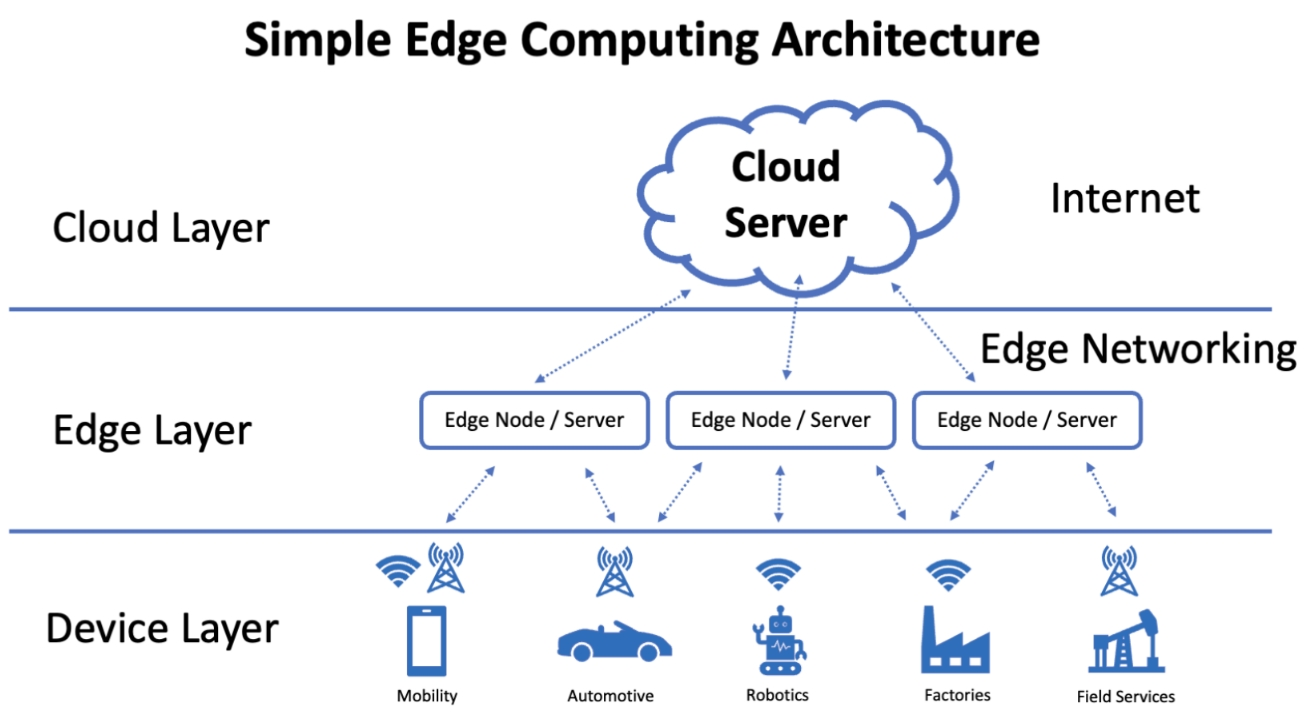
\includegraphics[width=1\textwidth]{images/edge_arch.jpg}
    \caption{Скица уобичајене \textit{edge} архитектуре}
    \label{fig:edge_arch}
\end{figure}

\subsection{Могуће примене}

Локалност, брзина и безбедност израчунавања \textit{edge computing}-a може бити од користи у разним случајевима:

    \subsubsection{Предикитвно одржавање машина у погонима} Неочекивани отказ машинa у индустријским погонима може значајно угрозити рад, профит фирме као и безбедност радника који њима управљају или се налазе у њиховој близини. Тренутни, најчешћи начин превеницје отказа оваквих машина обаваља се редовним, заказаним контролама и сервисима. Овакав приступ превенцији се показао као ефикасан, али његов проблем је што тешко и једино искуствено може одредити интервал између две контроле што резултује сувише честим или ретким контролама, што може довести до ненаданог престанка рада машине или узалудног губитка ресурса на сувишне контроле. \textit{Edge computing} овај проблем решава константим праћењем рада и стања сваке појединачне машине у реалном или приближно реалном времену помоћу мноштва сензора који су повезани или интегрисани у машине. На овај начин нема потребе за нагађањем времена контроле или поправке машине, због тога што се информације о стању машине могу добавити у било ком тренутку и по потреби организовати њихово сервисирање.

    \subsubsection{Видео надзор подржан вештачком интелигенцијом}

    Видео надзор је један од најраспрострањенијих начина константног удаљеног надзора, добављања информација, као и превенције нежељених догађаја. Све већим развојем вештачке интелигенције, могућности видео надзора се проширују са пуког посматрања снимака камера од стране човека на ауто детекцију објеката и препознавање значајних догађаја, попут уласка непознатих лица у објекат или присуства човека у деловима погона који могу угрозити његово здравље или живот. Оваква примена вештачке интелигенције захтева обраду података у реалном времену, као и конекцију са одређеним базама података и серверима који када би се налазили на \textit{cloud} платформама не би успевали да постигну најбоље перформансе и случајеви нестанка интернет конекције доводили би до потпуног отказа система. Због ових потешкоћа \textit{edge computing} је добар кандидат за имплементацију ових система због своје локалности уређаја за обраду података која смањује вероватноћу велике латенције и отказа комуникације између компоненти система.

    \subsubsection{Пренос догађаја уживо}

    Видео преноси утакмица, конференција и осталих догађаја временом добијају на квалитету што све више и више оптерећује њихов мрежни пренос. Закшњење које се јавља може представљати проблем гледаоцима који се налазе у непосредној близини самог догађаја. С тога се уместо слања на централни \textit{cloud} сервер, видео садржај поставља на локално распоређене \textit{edge} сервере којима гледаоци могу приступити са веома малом латенцијом.    
\pagebreak

\section{\textit{Fog computing}}

Иако се \textit{edge} и \textit{fog computing} често спомињу у истом контексту и неретко користе као синоними, постоји значајна разлика између ова два појма. \textit{Fog computing} представља унапређење \textit{edge computing}-а проширујући његове могућности обраде и складиштења података увођењем \textit{fog} чворова који се налазе између \textit{edge} и \textit{cloud} система. У суштини, он је екстензија \textit{cloud}-а с тиме да је много ближи уређајима \textit{edge} система \ref{fig:fog_arch}, што великим делом очувава све погодности \textit{edge computing}-а као што су брза мрежна комуникација, мала латенција и безбедност, а опет омогућава обраде података које захтевају много веће рачунарске ресурсе. Овако \textit{edge} систем још увек може самостално да обрађује најкритичније податке по безбедност и брзину рада апликације, а да остатак посла делегира \textit{fog} чворовима. Још једна од погодности је могућност много већег географског распростирања једног система користећи горе поменуте \textit{fog} чворове. 

\begin{figure}[H]
    \centering
    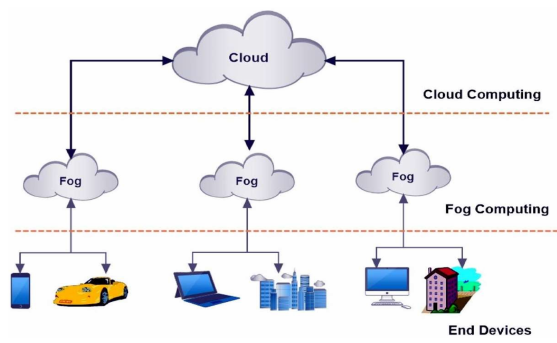
\includegraphics[width=1\textwidth]{images/fog_arch.png}
    \caption{\textit{Fog} је попут \textit{cloud}-а који је много ближи крајњим уређајима}
    \label{fig:fog_arch}
\end{figure}

\pagebreak
\subsection{Архитектура}

Архитектура \textit{fog computing}-a састоји се из шест слојева \ref{fig:fog_layers}:

\begin{figure}[H]
    \centering
    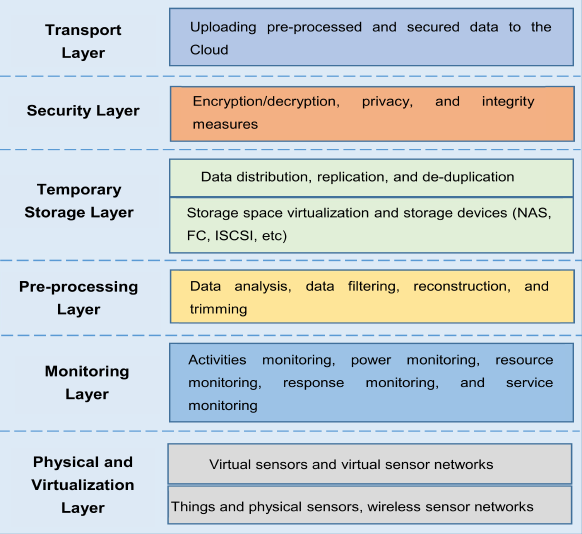
\includegraphics[width=1\textwidth]{images/fog_layers.png}
    \caption{Слојевита архитектура \textit{fog computing}-a}
    \label{fig:fog_layers}
\end{figure}

Физички и виртуелизациони слој укључује различите типове чворова попут физичких, виртуелних чворова или виртуелних сензорских мрежа. Различити чворови географски су дистрибуирани да би прикупили информације из њихове околине и послали их вишим слојевима уз помоћ \textit{gateway}-a на даље филтрирање и процесирање.

Слој за надзор прати искоришћење ресурса, доступност сензора и \textit{fog} чворова, као и осталих елемената мреже. Сви задаци које обављају чворови се прате у овом слоју, пратећи који чвор обавља који задатак, у које време, и шта ће му бити потребно у наредном кораку. Прате се перформансе и статус свих апликација и услуга које су имплементиране унутар система. Додатно, прати се и потрошња енергије \textit{fog} чворова.

У пре-процесном слоју сакупљени подаци се анализирају, врши се филтрирање и редуковање података како би се извукле значајне информације. Претпроцесирани подаци се затим складиште у слоју за привремено складиштење. Када се подаци пренесу на \textit{cloud}, више им није потребно локално складиштење и могу бити уклоњени са привремених складишних медија.

Безбедносни слој врши шифровање и дешифровање података, а често и примењује мере заштите њиховог интегритета, како их потенцијални нападачи не би могли неприметно прочитати или изменити приликом њиховог транспорта на \textit{cloud}.

На самом крају, у транспортном слоју, претпроцесирани подаци се транспортују на \textit{cloud} како би се издвојили и креирали додатни корисни сервиси. Ради ефикасне употребе енергије и очувања безбедности података, само део сакупљених података се транспортујe на \textit{cloud}. 

\subsection{Могуће примене}

Тренутна централизована архитектура \textit{cloud computing}-a суочава се са озбиљним изазовима за \textit{IoT} апликације. На пример, не може да подржи временски осетлљиве \textit{IoT} апликације, као што су \textit{video streaming, gaming} и \textit{augmented reality}. Такође, недостаје свест о локацији процеса, јер је у питању централизовани модел. \textit{Fog computing} може да реши ове изазове. \textit{Fog computing} делује као мост између \textit{IoT} уређаја и великих \textit{cloud} рачунарских и складишних услуга. Он пружа високо виртуализовани модел рачунања, складиштења и мрежних ресурса између крајњих уређаја и класичних \textit{cloud} сервера.

\subsubsection{Аутономна возила}

Постоје многе корисне функционалности, које зависе од \textit{fog}-a и интернет конекције, које могу бити додате аутомобилима као што су "\textit{hands free}" режим вожње или функција самопаркирања која више не би захтевала возача за воланом како би се аутомобил паркирао.
У следећих неколико година се очекује да ће сви нови аутомобили имати могућност комуникације са блиским аутомобилима и интернетом. \textit{Fog computing} ће бити најефикасније решење за сва возила повезана са интернетом, јер омогућава комуникацију у реалном времену. Такође, омогућиће аутомобилима, приступним тачкама и семафорима да комуницирају једни са другима како би обезбедили добру услугу корисницима.
Уз коришћење \textit{fog}-a уместо \textit{cloud}-a, судари и другe несреће могле би се свести на минимум.

\subsubsection{Паметне куће}

\textit{IoT} има многo повезаних сензора и уређаја унутар домаћинстава. Међутим, ови уређаји долазе од различитих произвођача и користе различите платформе, што отежава њихово међусобно повезивање. Такође, неки задаци захтевају велику количину рачунарских ресурса и простора за складиштење података. \textit{Fog computing} решава многе од ових проблема, интегрише све различите платформе и омогућава паметним кућним апликацијама приступ флексибилним ресурсима. \textit{Fog computing} такође пружа много предности за апликације за обезбеђивање домаћинстава.   
\pagebreak

\section{\textit{Continuum computing}}

\textit{Continuum computing} представља еволуцију претходно поменутих парадигми, интегришући  \textit{edge, fog} и \textit{cloud computing} у један кохезиван динамички систем, трудећи се да усклади локализовани \textit{edge}, средишњи \textit{fog} и централизовани \textit{cloud} пружајући споља кориснику једну јединствену, свеприсутну мрежу уређаја, олакшавајући му коминикацију и интеракцију без потребе за размишљањем о сложености позадинске технологије. Чине га мноштво разноликих уређаја попут мобилних уређаја, сензора и  \textit{IoT} уређаја.

Интегришући ресурсе \textit{cloud}-a, \textit{edge} уређаје и \textit{IoT}, \textit{continuum computing} омогућава ефикасне, \textit{real time} и динамичке рачунске процесе који задовољавају потребе данашњих разноврсних апликација. Он обавља рачунске операције дистрибуирајући оптерећење преко више уређаја у систему. Сваки уређај обавља део посла, а резултати се комбинују како би се произвео крајњи резултат. Ово омогућава брже време обраде и повећану скалабилност. Са \textit{continuum computing}-ом, рачунске операције се ефикасно обављају прилагођавајући се променљивим захтевима и оптимизујући искоришћеност ресурса ван традиционалних граница. Ова алокација ресурса се заснива на факторима као што су близина ресурса, рачунарска способност и давање приоритета задацима који захтевају брзу реакцију. У зависности од задатка, одговори у реалном времену могу бити пренесени на \textit{edge} уређаје, док се комплексна аналитика подразумевано може обавити у \textit{cloud}-у. Ова динамичка дистрибуција задатака побољшава перформансе система и ефикасност обраде док смањује латенцију. Општа архитектура \textit{continuum computing}-а је приказана на слици \ref{fig:continuum_arch}.

\begin{figure}[H]
    \centering
    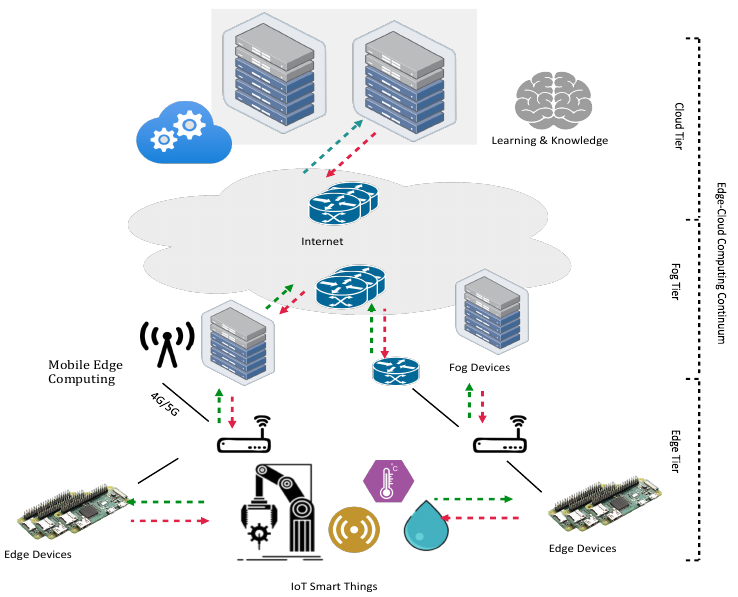
\includegraphics[width=1\textwidth]{images/continuum_arch.png}
    \caption{Архитектура \textit{continuum computing}-а}
    \label{fig:continuum_arch}
\end{figure}

Агилност овакве архитектуре доноси многе предности укључујући  оптимизацију мрежног протока, скалабилност, малу латенцију, ефикасно искоришћене ресурса, балансирање оптерећења, флексибилност и поузданост. Упркос свим овим предностима, наилази се и на одређене потешкоће и изазове као што су међусобна комуникација уређаја различитих произвођача који функционишу служећи се различитим семнатичким правилима, сложеност управљања великог броја уређаја и синхорнизација података.

\pagebreak
\subsection{Могуће примене}

\subsubsection{Паметни градови}

Паметни град користи мрежу сензора и уређаја за прикупљање информација у реалном времену о транспорту, потрошњи енергије, управљању отпадом и јавним услугама. Подаци са ових извора могу се анализирати и користити за донoшење одлука, као средство за повећање комфора, унапређење јавних услуга и квалитет живота грађана. Пошто \textit{continuum computing} има подразумевану скалабилност, он се  може динамички повећавати или смањивати као одговор на промене у екосистему паметног града.

\subsubsection{Здравство}

Здравство обухвата различите медицинске услуге, технологије и системе који су дизајнирани да спрече, дијагностикују, лече и управљају болестима и здравственим стањима. У последњих неколико година развијено је  неколико медицинских уређаја, од мобилних сензора до високопрофесионалних машина (постављених у болницама и здравственим центрима) који се користе за прикупљање података о пацијентима и њихово процесирање путем паметних телефона или у \textit{cloud}-у. Здравствена индустрија захтева тачне и брзе аналитичке резултате од рачунарских уређаја. Понекад је неопходно анализирати захтевне задатке као што су медицински снимци (рентген или ЦТ снимци) или геномско секвенцирање, али се резултат очекује у кратком временском периоду. Понекад је потребно користити вештачку интелигенцију или машинско учење за предвиђање стања пацијента, што захтева више рачунарских ресурса.   
\pagebreak

\section{Закључак}
 
У овом семинарском раду, истраженe су архитектуре система великих скупова података којe обухватају \textit{Edge, Fog} и \textit{Continuum computing}. Свака од ових парадигми има своје јединствене карактеристике и примене у модерном дигиталном окружењу.

\textit{Edge computing} се фокусира на обраду података крај самог извора, што доводи до смањења латенције и бољег одзива за крајње кориснике. Онo омогућава примену специфичних алгоритама и решења на уређајима на месту самих података.

\textit{Fog computing} нуди додатни слој за процесну обраду између уређаја на рубу мреже и централизованих \textit{cloud} система. Овaкав приступ побољшава скалабилност и могућност ресурсно захтевне анализе података пре њиховог слања на \textit{cloud}, што је посебно значајно у условима великог броја података и аналитички захтевних задатака.

\textit{Continuum computing} представља еволуцију ових парадигми интегришући их у кохезиван динамички систем. Он омогућава усклађивање локализованoг \textit{edge}-а, средишњег \textit{fog}-а и централизованог \textit{cloud-а}. Оваква интеграција отвара врата за унапређене могућности обраде података, побољшавање ефикасности мрежа и оптимизацију ресурса.

Захваљујући овим технологијама, предстојећи развој информационих система имаће значајне користи у областима као што су \textit{IoT}, мобилна комуникација, паметни градови, индустрија и здравствo. 
\newpage
\newpage

\section{Библиографија}

\begin{enumerate}
    \item \href{https://link.springer.com/article/10.1007/s00607-022-01104-2}{Edge computing, A grounded theory study}
    \item \href{https://www.ericsson.com/en/reports-and-papers/white-papers/edge-computing-and-deployment-strategies-for-communication-service-providers}{Edge computing and deployment strategies for communication service providers}
    \item \href{https://www.redhat.com/en/resources/bring-insight-data-customer-edge-computing-whitepaper}{Edge computing brings data and insight closer to customers}
     \item \href{https://www.researchgate.net/publication/341096184_An_Overview_on_Edge_Computing_Research}{An Overview on Edge Computing Research}
    \item \href{https://www.mdpi.com/2504-2289/2/2/10}{Fog Computing and the Internet of Things: A Review }
    \item \href{https://www.mdpi.com/2073-431X/12/10/198}{Exploring the Potential of Distributed Computing
Continuum Systems}
    \item \href{https://www.mdpi.com/2078-2489/14/3/198}{Fundamental Research Challenges for Distributed Computing
Continuum Systems}
\item \href{https://picture.iczhiku.com/resource/paper/WhIeGHQRAPDTfxCC.pdf}{Cloudlets: Bringing the cloud to the mobile user}
\item \href{https://journal.uob.edu.bh/bitstream/handle/123456789/4584/IJCDS_120105_1570717273.pdf?sequence=3&isAllowed=y}{Fault Tolerance Mechanism for Software Application Through
Fog Computing as Middleware}
\end{enumerate} 
% \bibliographystyle{plain}
% \typeout{}
% \bibliography{biblist}

\end{document}